\section{Results}
\label{sec:results}

Our main result is the comparison of compiled circuit sizes and depths between 
normal Solovay-Kitaev and Super-Kitaev as shown in the Figure
\ref{fig:size-depth}. In the graph legend, ``Super'' referes to Super-Kitaev
and ``Normal'' refers to Solovay-Kitaev.
Solovay-Kitaev in the worst case has identical
The discrete steps in Solovay-Kitaev's circuit size and depth are due
to the levels of recursion, which are conservatively chosen to meet
the desired precision. The initial step reflects the fact that even
before successive approximation, our initial generated sequences
(basic approximations in Section \ref{sec:sk-algo}) already meet large
desired precisions. As expected, Super-Kitaev's depth compares very
favorably with Solovay-Kitaev.
The graphs are roughly linear in a log-log plot, with a non-linearity
for low precisions due to irregularities in the adder circuits for small
$n$.

\begin{center}
\begin{figure}[h!]
\label{fig:size-depth}
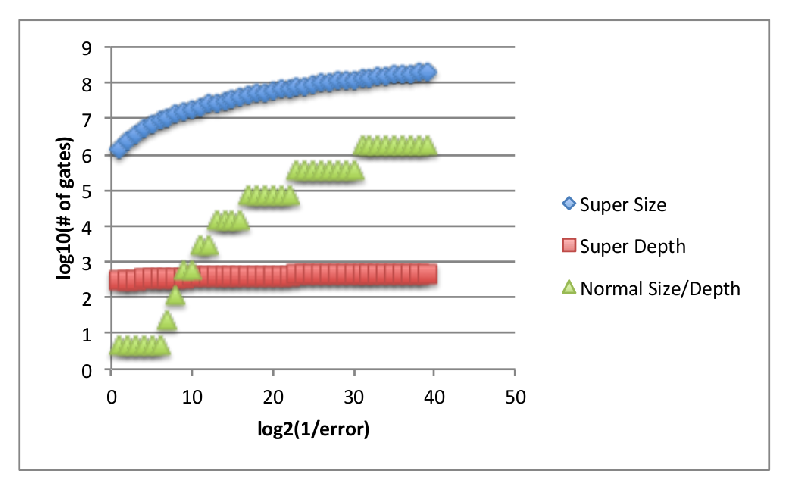
\includegraphics[width=3in]{circuit-size-depth.eps}
\caption{Compiled circuit size and depth}
\end{figure}
\end{center}

The tradeoff between Solovay-Kitaev and Super-Kitaev can most clearly
be seen in the use of space. Solovay-Kitaev uses no ancillae at run-time,
but requires a classical preprocessing step to generate basic
approximations (precompiled sequences from the universal set). Although
we did not generate sequences beyond $l_0 = 9$ for $SU(4)$, the curve
indicates it would soon require terabytes of storage, even if a more
efficient encoding were used (e.g. programming in C instead of Python).
Super-Kitaev, on the other hand, requires no preprocessing space, but
has a (currently intractable) requirement for ancilla qubits are run-time
which tracks the circuit size as $O(n^2 \log n)$.

\begin{center}
\begin{figure}[h!]
\label{fig:generation}
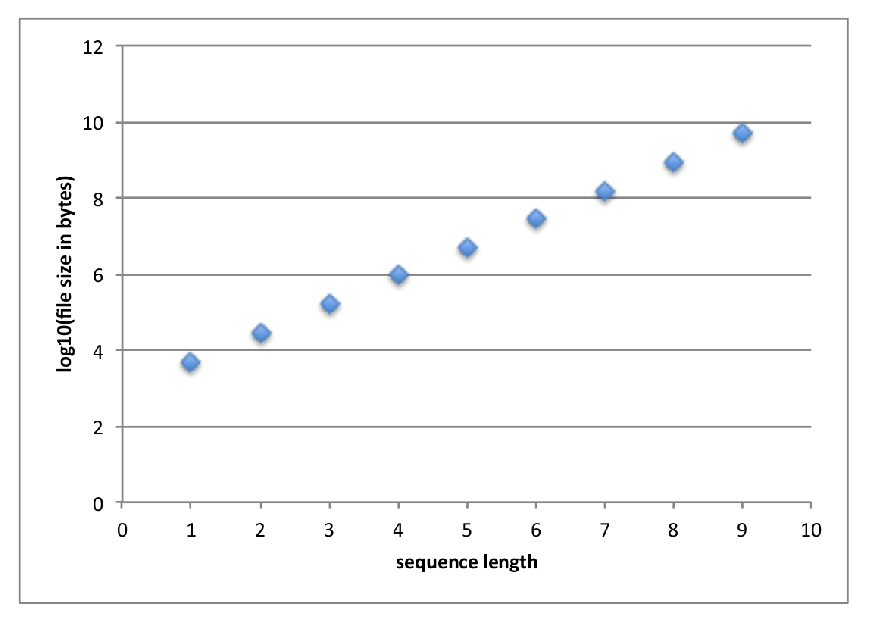
\includegraphics[width=3in]{normal-generation.eps}
\caption{Solovay-Kitaev preprocessing file sizes}
\end{figure}
\end{center}

\begin{center}
\begin{figure}[h!]
\label{fig:ancilla}
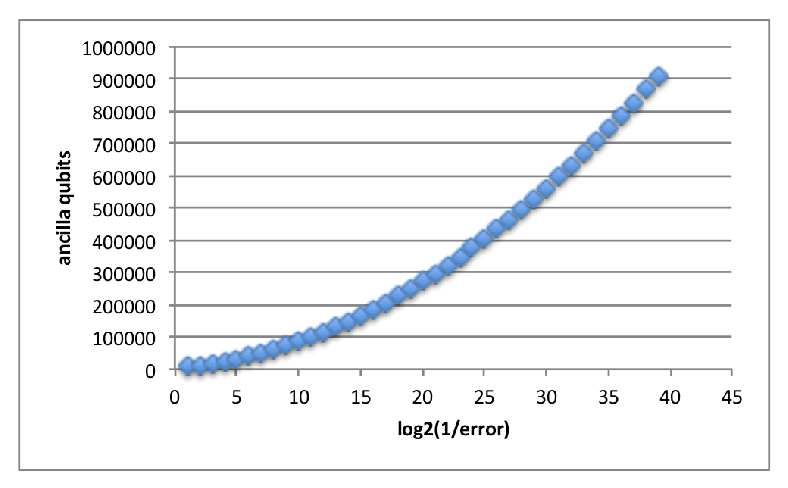
\includegraphics[width=3in]{super-ancilla.eps}
\caption{Super-Kitaev ancilla}
\end{figure}
\end{center}
